\chapter{Structure of CoCos}

\section{Description of CoCos}

The structure of a CoCo is characterized by two components: the trigger mechanism which initializes the conversion of debt into equity and the loss absorption mechanism which determines the write-down or the conversion in shares. A brief overview c

\begin{figure}[ht]
	\centering
	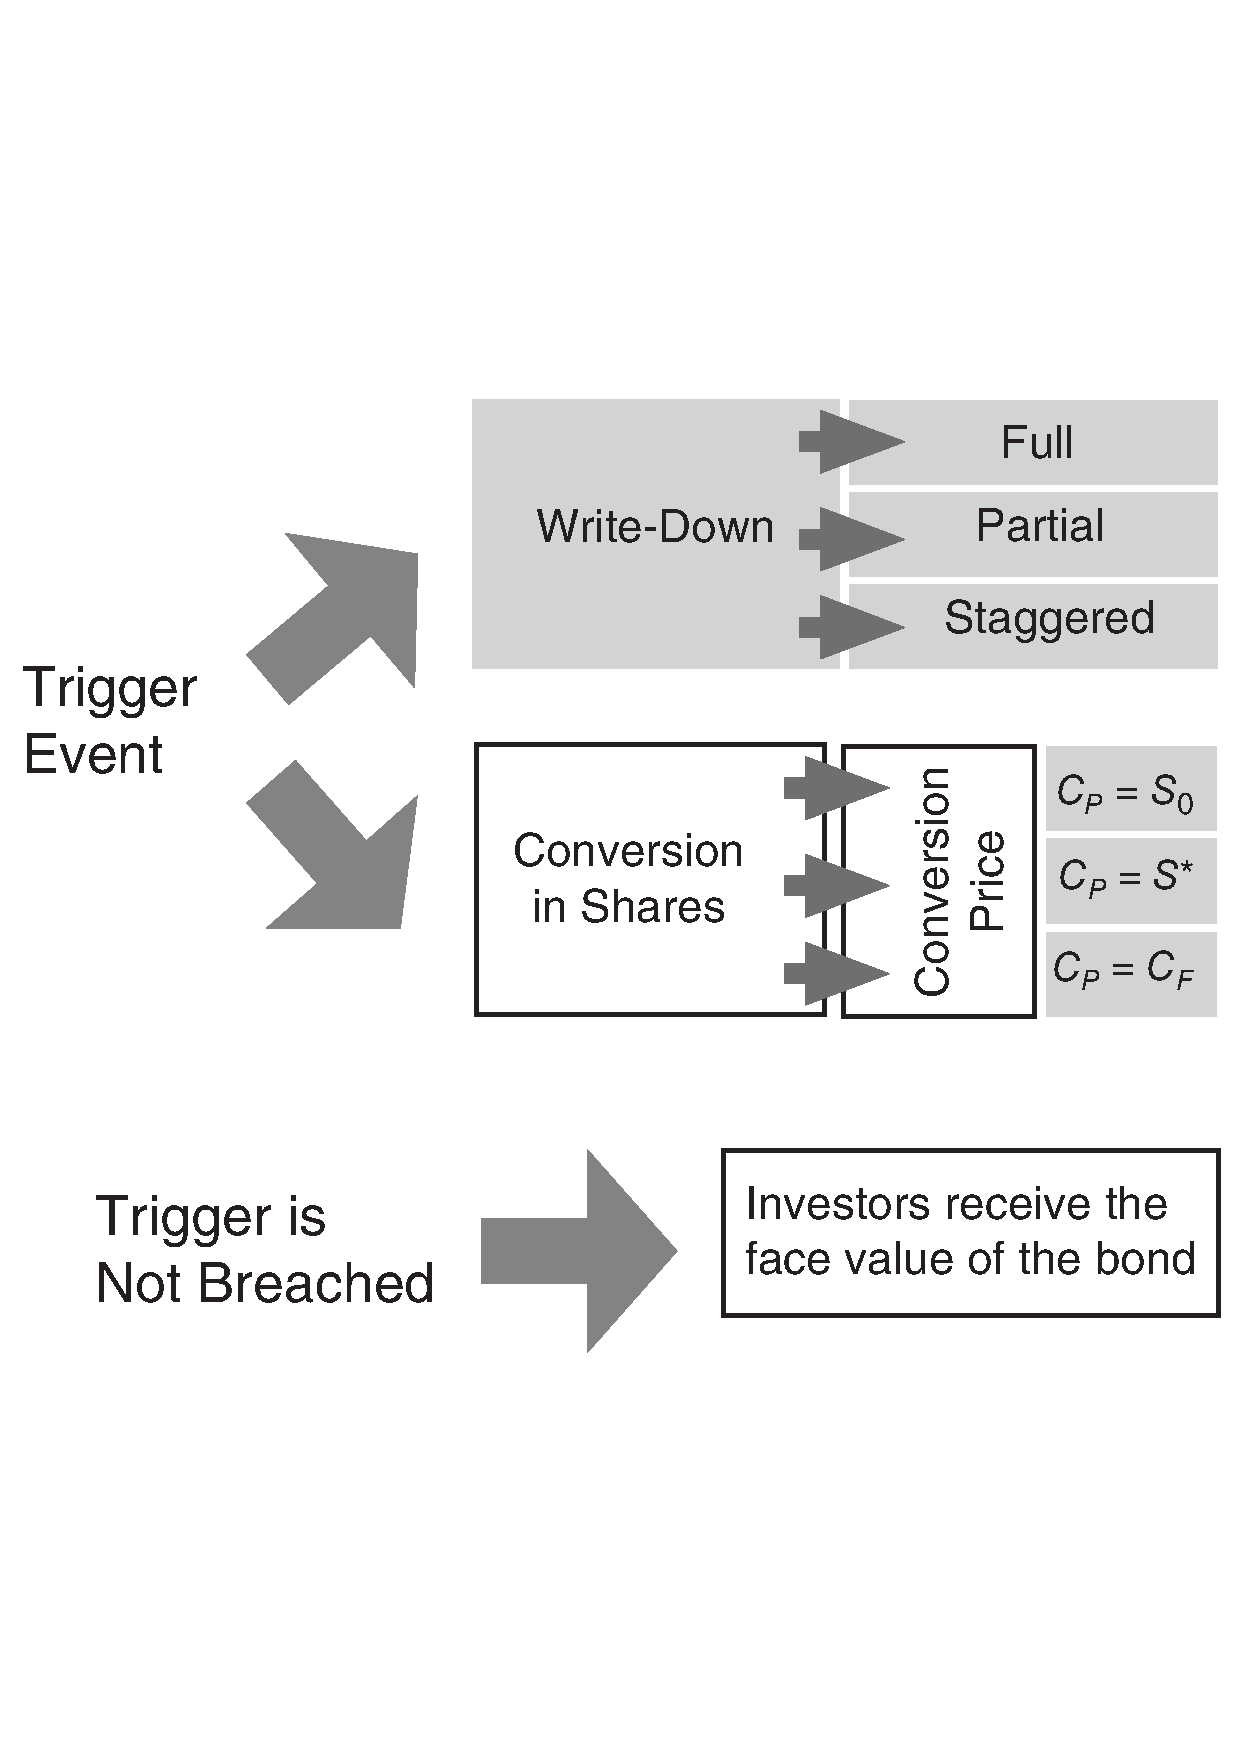
\includegraphics[trim=0.6cm 7.05cm 0.9cm 7cm, scale = 0.4]{media/anatomy} \par
	\caption[Anatomy of CoCos]{Anatomy of CoCos \citep{de2014handbook}}
\end{figure}

%\begin{figure}[ht]
%	\centering
%	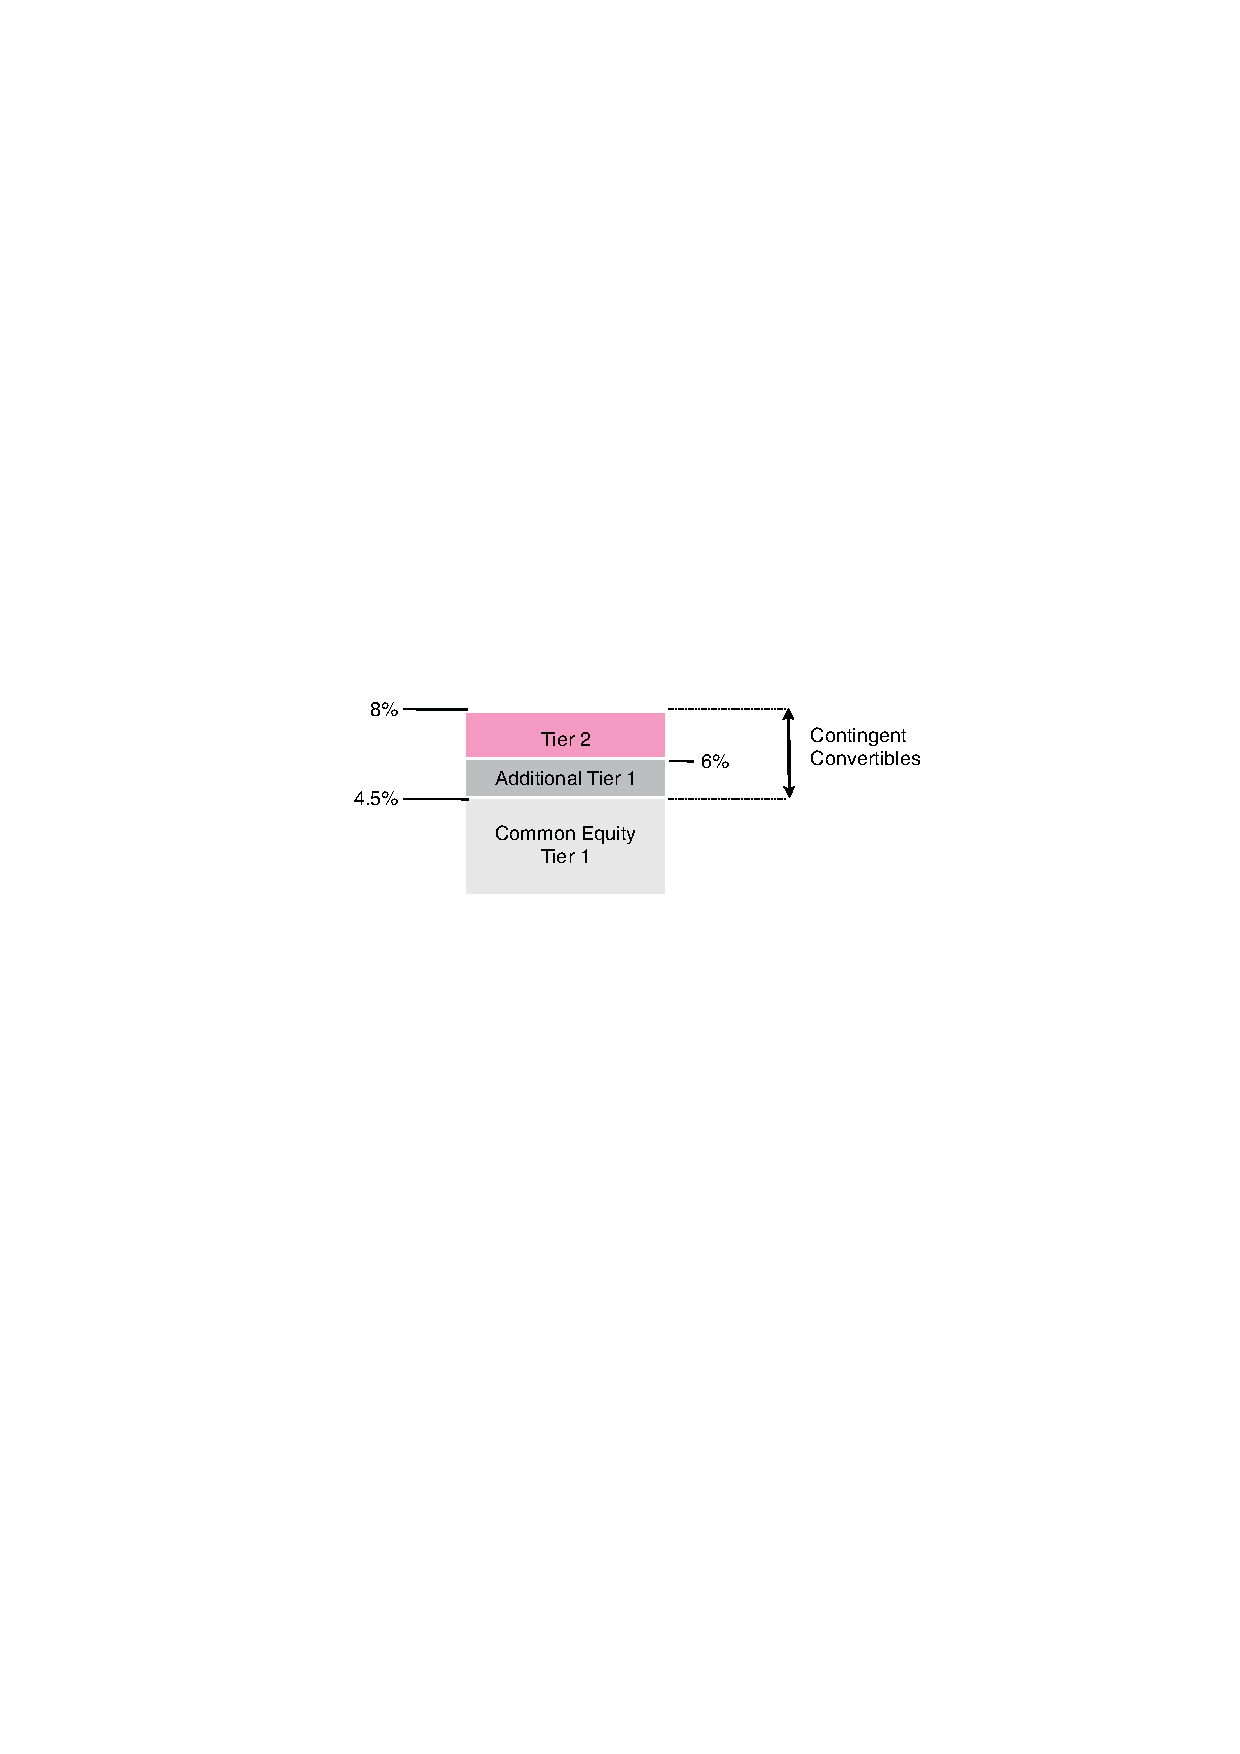
\includegraphics[trim=0.1cm 0.1cm 0.2cm 0.1cm, scale = 1]{media/basel3} \par
%	\caption[CoCos under Basel III]{CoCos under Basel III \citep{de2014handbook}}
%\end{figure}

\section{Payoff and Risk Profile}

\section{Trigger Mechanism}

The trigger is a key design element of a CoCo. In the following section, four different trigger mechanisms will be evaluated based on general design factors as summarized by \citet{erismann2015pricing}. The accounting trigger will be illustrated in section \ref{accountingtrigger} followed by the market trigger in section \ref{markettrigger}. Additionally, the regulatory trigger will be detailed in section \ref{regulatorytrigger} and the multi-variate trigger will be explained in section \ref{multivariatetrigger}. Hereinafter, the trigger types will be evaluated based on the following criteria:

\begin{itemize}
\renewcommand\labelitemi{--}
\item \textbf{Clarity}:  The trigger mechanism should be universally applicable irrespective of the jurisdiction in which the CoCo is traded.
\item \textbf{Fixedness}: The definition of a CoCo's trigger should remain the same until maturity.
\item \textbf{Frequency}: Data to which the trigger is linked should be updated at frequent intervals.
\item \textbf{Objectiveness}: The trigger mechanism should be based on observable and well-known facts. Their should be no room for subjectivity.
\item \textbf{Publicity}: Data should be open to the general view of all market participants. This needs to be possible without concealment. 
\item \textbf{Transparency}: The trigger mechanism should have the property that investors can see it publicly, thereby reducing the chance of manipulation.
\end{itemize}

\subsection{Accounting Trigger}\label{accountingtrigger}

CoCos with accounting trigger have a loss absorption mechanism which is inherently connected to the financial soundness of a bank's balance sheet. Accounting triggers are built upon capital ratios which compare a bank's regulatory capital with its assets. Conversion occurs if a pre-determined metric falls below a certain threshold. Hence, capital ratios are an objective indicator for a bank's solvency as they are defined uniformly for all financial institutions by regulatory authorities. \citep{de2014handbook} \citet{pazarbasioglu2011contingent} note that accounting triggers are easy to price, intuitive and simple to implement. Issuing banks and regulators seem to have perceived the benefits of accounting triggers partly because a significant portion of CoCos use the common equity tier (CET1) ratio as reference metric. Examples of CoCos will be described shortly in section \ref{cocoexamples}.\\

That said, objections against accounting triggers follow the line of thought that they just become active long after the need for loss absorbing capital arose. One might argue that accounting triggers assess the viability of financial institutions from a perspective that is far-removed from reality. \citep{de2011pricing} Moreover, as accounting concept, book values are prone to manipulation and managerial dishonesty especially in times of distress. \citep{mcdonald2013contingent}\\ 

Empirical findings bring up a further aspect. \citet{haldane2011capital} points out that major financial institutions, which either went bankrupt, were bailed out or were taken over under distress during the global financial crisis, reported similar CET 1 ratios right before the collapse of Lehman Brothers compared to their peers which coped relatively well with the collapse of the financial system. In this context, \citet{haldane2011capital} highlights that market-based solvency measures\footnote{\citet{haldane2011capital} mentions three metrices: (1) market-based capital ratio (ratio of market capitalization to total assets), (2) market-based leverage ratio (ratio of market capitalization to total debt) and (3) Tobin's Q (ratio of market capitalization to book value of equity).} performed creditably as they showed clear signals of impending distress a year ahead of the bankruptcy of Lehman Brothers. Empirical evidence of \Citet{valukas2010report} further supports these findings. This leads to the conclusion that CoCos with accounting triggers might not reinforce distressed banks at the right time but instead produce more false positives, which means that CoCos of non-distressed banks trigger prematurely. Inefficiencies like higher funding costs could be the consequence. \citep{pazarbasioglu2011contingent}

\subsection{Market Trigger} \label{markettrigger}

A market trigger uses directly observable indicators like the issuing company's share price or credit default swap (CDS) spreads while assuming sufficiently efficient markets. The major advantage of those measures is that one can observe and verify them in real-time. \citep{haldane2011capital} Market triggers are widely discussed in academia and seen as preferable trigger mechanism. \citet{calomiris2013design} pronounce themselves for using share prices. Besides, \citet{haldane2011capital} and \citet{pazarbasioglu2011contingent} contend to apply market-based capital ratios as trigger indicator. Their line of argumentation is based on some of the best-known examples of corporate defaults, which were indicated well before by a serious and continuous deterioration of a company's market capitalization.\\ 

This also applies to the aforementioned example of Lehman Brothers. If the bank had been obliged to issue CoCos with a trigger directly linked to its share price the decline in equity value would have triggered the conversion in due time.\citep{calomiris2013design} Hence, the bankruptcy could have been prevented with a CoCo. However, practitioners argue that it comes at a risk to use market data as reference because markets are prone to manipulation. Moreover, self-fulfilling prophecies of share price dilution could lead to downward spirals that ultimately lead to CoCo conversions. \citep{pazarbasioglu2011contingent} The severity of the aforementioned argumentation can be attentuated by using moving averages, which are less susceptible to manipulation. 

\subsection{Regulatory or Non-Viability Trigger} \label{regulatorytrigger}

Regulatory or non-viability trigger is a conversion mechanism by which a CoCo is converted into equity at the discretion of the responsible supervisory authority. The rationale behind this approach is that regulators want to limit the impact of any development that could pose a danger to the going-concern of a systemically important bank.\citet{erismann2015pricing} Moreover, this kind of trigger would eliminate the periodicity problem of accounting data and the risk of market manipulation.\\ 

Though, it is very difficult for market participants to estimate the conversion probability of a CoCo with regulatory trigger. The valuation of such a hybrid instrument becomes opaque for market participants with limited information. \citep{alvemar2012modelling} One can also argue that a CoCo's marketability is weakened because of the greater uncertainty which could ultimately lead to higher funding costs. \citep{de2014handbook} 

\subsection{Multi-Variate Trigger} \label{multivariatetrigger}

The multi-variate trigger uses a combination of the aforementioned trigger mechanisms. It extends the accounting trigger of a CoCo by a universal regulatory trigger which covers severe states of the world adversely impacting the stability of the financial system. In this context, the \citet{squam2009expedited} supports the implementation of this dual trigger mechanism as it combines the best of two worlds. On the one hand, the bank-specific trigger serves as disciplining mechanism for a bank's management. It reduces the political pressure from the regulator who has to decide whether the systemic trigger is met. Second, if the conversion of a CoCo is only linked to a systemic trigger, even well capitalized banks would be forced to convert debt into equity during a systemic crisis. This would disincentivize financially sound banks to preserve their status quo.

\subsection{Evaluation of Trigger Types}
Generally, one can evaluate the aforementioned trigger types based on the design criteria as stated in the beginning.

\begin{table}[H]
	\setlength{\extrarowheight}{2.5pt}
	\centering
	\begin{tabular}{lcccc}
		\toprule
			 & Accounting & Market & Regulatory & Multi-Variate \\
		\midrule
			Clarity & medium & high & low & medium\\
			Fixedness & high & high & low & high \\
			Frequency & medium & high & low & high\\
			Objectiveness & medium & high & low & medium \\
			Publicity & high & high & high & high \\
			Transparency & medium & high & low & medium \\
		\bottomrule
	\end{tabular}
	\caption[Evaluation of different trigger mechanisms]{Evaluation of different trigger mechanisms based on design criteria. The status high means that the trigger type meets the requirements, whereas low implies that it does not satisfy the conditions. \citep{erismann2015pricing}}
	\label{table:evaluationtrigger}
\end{table}

We see in table \ref{table:evaluationtrigger} that the market trigger is a preferable mechanism as it fulfills all important design criteria. Furthermore, one has to take into account that \citet{haldane2011capital} described that market trigger were historically the preferable mechanism as it served as early-warning indicator. In section \ref{examples} different CoCos will be highlighted with their design elements also covering their trigger mechanism. This is a good way to understand whether banks and regulators followed the aforementioned rationale.

\section{Loss-Absorption Mechanism}

\begin{itemize}
\item on the appearance of trigger event at a trigger moment, the bond can be either convert into shares or receive a haircut on its face value $N$
\end{itemize}

\subsection{Conversion into Shares}
\begin{itemize}
\item number of shares received per converted CoCo is the conversion rate $C_r$, which is normally determined ex-ante
\item the conversion amount $\alpha N$ is determined by the conversion fraction $\alpha$ and the face value $N$
\item the implied concersion price $C_p$ is
\end{itemize}

\begin{align}
C_p &= \frac{\alpha N}{C_r}
\end{align}

\begin{itemize}
\item recovery rate $R_{CoCo}$ is determined by the share price $S^*_T$ divided by the conversion price $C_p$
\begin{itemize}

\begin{align}
R_{CoCo} &= \dfrac{S^*_T}{C_p}
\end{align}

\begin{itemize}
\item if the bond is converted into shares, the loss for the investor $L_{CoCo}$ depends on the conversion ratio $C_r$ and the value $S^*$ of the shares at time $t$ when the trigger materializes
\end{itemize}

\begin{align}
L_{CoCo} &= N - ( 1 - R_{CoCo}) = N \left( 1 - \frac{S_T^{*}}{C_p} \right)
\end{align}

\begin{itemize}
\item the equivalent final payoff $P_T$ is equal to
\end{itemize}

\begin{align}\label{valueatmaturity}
    P_T &= \begin{cases} (1 - \alpha) N + \frac{\alpha N}{C_p} S_T^{*} & \text{ if converted} \\ N & \text{if not converted} \end{cases}

\subsection{Write-Down}

\section{Conversion Details}


\chapter{CoCo Examples} \label{cocoexamples}

\section{Examples} \label{examples}

